%! TEX program = lualatex
% For exporting as word use:
% pandoc -s apodemus-vacc-main.tex --filter pandoc-crossref --citeproc --csl nature.csl --bibliography=apodemus-vacc-refs.bib -o ../Venkatesan_et_al_R1.docx

\documentclass[a4paper, hidelinks, 11pt]{article}

%%%%%%%%%%%%%%%%% LOAD PACKAGES %%%%%%%%%%%%%%%%
\usepackage[british]{babel}
\usepackage{microtype}

% font settings
\usepackage{fontspec}
\usepackage{mathtools}
\usepackage{textcomp}
\usepackage{eurosym}
\usepackage{unicode-math}
\usepackage{MnSymbol} % provides independence symbol
\usepackage{lipsum}

\defaultfontfeatures{Ligatures=TeX}

\setmainfont[
    Extension=.otf,
    UprightFont= *-regular,
    BoldFont=*-bold,
    ItalicFont=*-italic,
    BoldItalicFont=*-bolditalic,
    ]{TeX Gyre Pagella}

\setsansfont[
        Extension=.otf,
        UprightFont= *-regular,
        BoldFont=*-bold,
        ItalicFont=*-italic,
        BoldItalicFont=*-bolditalic,
        ]{TeX Gyre Heros}

\setmathfont{TeX Gyre Pagella Math}

\setmonofont{IBM Plex Mono Text}
% \setmonofont{TeX Gyre Cursor}[Scale=1]

% headings
\usepackage{titlesec}

\titleformat*{\section}{\large\bfseries\sffamily\MakeUppercase}
\titleformat*{\subsection}{\normalsize\bfseries\sffamily}
\titleformat*{\subsubsection}{\normalsize\bfseries\sffamily}
\titleformat*{\paragraph}{\normalsize\bfseries\sffamily}
\titleformat*{\subparagraph}{\normalsize\bfseries\sffamily}

% \titlespacing\section{0pt}{12pt plus 4pt minus 2pt}{0pt plus 2pt minus 2pt}
% \titlespacing\subsection{0pt}{12pt plus 4pt minus 2pt}{0pt plus 2pt minus 2pt}
% \titlespacing\subsubsection{6pt}{12pt plus 4pt minus 2pt}{0pt plus 2pt minus 2pt}
\titlespacing\paragraph{12pt}{0pt plus 4pt minus 2pt}{4pt plus 2pt minus 2pt}

% page setup
\usepackage{titling} % to use \maketitle more than once
\usepackage{fancyhdr}
\usepackage{authblk}
\usepackage{booktabs} % For prettier tables
\usepackage{color}
\usepackage{lineno}
% \modulolinenumbers[5]
\usepackage{csquotes}
\linenumbers

% Text alignment (comment out for fully justified)
% \usepackage[document]{ragged2e}

% prevent widows and orphans
\usepackage[defaultlines=2,all]{nowidow}
\usepackage{needspace}

% create outline and links in pdf
\usepackage{hyperref}
\usepackage[numbered]{bookmark}
\makeatletter
\renewcommand\@seccntformat[1]{}
\makeatother

% debug warnings
\overfullrule=1cm


%%%%%%%%%%%%%%%%% TABLES & FIGURES %%%%%%%%%%%%%%%%
% captions
\usepackage[labelfont=footnotesize,textfont=footnotesize,singlelinecheck=off,justification=raggedright]{subcaption}
\DeclareCaptionLabelSeparator{pipe}{\textrm{ | }}
\usepackage[figurename=Fig.,
            font={sf,footnotesize},
            labelfont=bf,
            labelsep=quad]{caption}

% figures:
\usepackage{graphicx}
\usepackage{wrapfig}
\usepackage{floatrow}
\usepackage{tikz}

% tables:
\usepackage{tabulary}
\usepackage{multirow}
\usepackage{ltablex}
\usepackage{longtable} % Note: It may be necessary to compile the document several times to get a multi-page table to line up properly
% \usepackage[table,xcdraw]{xcolor}
\usepackage{threeparttable}

%%%%%%%%%%%%%%%%% ANNOTATIONS %%%%%%%%%%%%%%%%
\usepackage{soul} % highlighting & strikeout
\setlength{\marginparwidth}{2cm} % make room for comments
\usepackage[colorinlistoftodos, textsize=tiny]{todonotes}

%%%%%%%%%%%%%%%%% BIBLIOGRAPHY %%%%%%%%%%%%%%%%
\usepackage[
    style=nature,
    sorting=none,
    backend=biber,
    ]{biblatex}
\addbibresource{apodemus-vacc-refs.bib}
\renewcommand*{\bibfont}{\sffamily\footnotesize}

%%%%%%%%%%%%%%%%% PAGE SETUP %%%%%%%%%%%%%%%%
\topmargin0.3cm
\oddsidemargin0.0cm
\textwidth15cm
\textheight22cm
\footskip1.3cm

\pagestyle{fancy}
\fancyhead{}
\fancyhead[RO]{\emph{Wild vaccines}}
% \fancyfoot[RO, LE]{\thepage{}}
\fancyfoot[c]{\thepage{}}

\setlength{\headheight}{14pt}
\renewcommand{\headrulewidth}{0.4pt}
\renewcommand{\footrulewidth}{0pt}

%%%%%%%%%%%%%%%%% TITLE PAGE %%%%%%%%%%%%%%%%

\title{Causes of variation in vaccine efficacy in a wild rodent population}

\author[1]{Saudamini Venkatesan}
\author[2]{Ewan Smith}
\author[1,\dag]{Amy B. Pedersen}
\author[2,\dag,*]{Simon A. Babayan} % 0000-0002-4949-1117

\affil[1]{Institute of Evolutionary Biology, University of Edinburgh, Scotland, UK, EH9 3JT}
\affil[2]{Institute of Biodiversity, Animal Health and Comparative Medicine, University of Glasgow, Glasgow, G12 8QQ, Scotland, UK,}
\affil[ \dag]{These authors contributed equally to this work}
\affil[*]{Corresponding authors: amy.pedersen@ed.ac.uk, simon.babayan@glasgow.ac.uk}

% \renewcommand\Authfont{\normalsize}
\renewcommand\Affilfont{\normalsize}

% Include the date command, but leave its argument blank.
\date{}

% Set title for the abstract (default is "Abstract")
\addto\captionsbritish{\renewcommand\abstractname{\vspace{-\baselineskip}}}

%%%%%%%%%%%%%%%%% END OF PREAMBLE %%%%%%%%%%%%%%%%

\begin{document}
% Import list of figures

% Double-space the manuscript.
\baselineskip24pt

% Don't number lines on title page
\nolinenumbers

% Make the title.
\maketitle

\listoftodos

\todo{Fix author list \& affiliations}

% Start numbering lines here
\linenumbers

\begin{abstract}

\noindent\bf\textsf{Individuals vary broadly in their response to vaccination and subsequent challenge infection, with poor vaccine responders causing persistence of both infection and transmission in populations.}

\end{abstract}

\textbf{Keywords:} Helminth; vaccine; immunoparasitology; machine learning; pathway analysis; ageing.

\pagebreak

\section{Outline}

Two main classes of vaccination: [AD, DA] vs [DD]. DD is the booster (can we rescue poor responders?). We are focussing on the variation within vaccine regimens: why do individuals vary despite identical vaccines?

Aims:

\begin{itemize}
    \item what drives variation in immune response?
    \item why do vaccine lose efficacy in the wild?
    \item can we recover the non-responders, with boosters, diet, other interventions\dots
    \item vaccination to probe wild immune systems
    \item methods development
\end{itemize}

\begin{enumerate}
    \item Partition differences between adjuvant and dose regimen
    \begin{itemize}
        \item Be clear that we chose alum to elicit type 2 antibody responses, because we can really only measure IgG1 in this system. Discussion: we might see different relationships between diet and antibody response if we measure other antibody isotypes.
        \item Comparison between AD, DA, DD
    \end{itemize}
    \item Total effects of interventions
    \begin{itemize}
        \item \(OD \sim V + W + D + V:W + V:D + W:D\) on all mice => plot of OD by Diet (D) and Lab vs Wild (W)
        \item \(OD \sim V + P + D + V:P + V:D + P:D\) on wild mice only
        \item Depending on the results of the models above, break down further.
    \end{itemize}
    \item Disentangling effects of environmental covariates with SCM: how do Sex, Weight, Parasite infection, reproductive status, and time since vaccination affect immunisation efficacy?
\end{enumerate}


\pagebreak
\section{Introduction}

Individuals vary widely in their responses to vaccination and little is known
about the causes underlying low vaccine efficacy, nor how effective a vaccine
will be ``in the real world'' against the pathogen for which it has been
developed.

\begin{figure}
    % This code uses the tikz package
    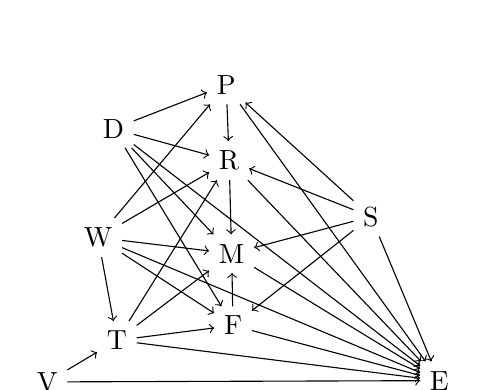
\begin{tikzpicture}[scale=1.5]
        \node (v0) at (-1.15,1.58) {D};
        \node (v1) at (1.61,-0.552) {E};
        \node (v2) at (-0.137,-0.0856) {F};
        \node (v3) at (-0.149,0.523) {M};
        \node (v4) at (-0.195,1.95) {P};
        \node (v5) at (-0.170,1.31) {R};
        \node (v6) at (1.03,0.836) {S};
        \node (v7) at (-1.12,-0.211) {T};
        \node (v8) at (-1.71,-0.563) {V};
        \node (v9) at (-1.28,0.659) {W};
        \draw [->] (v0) edge (v1);
        \draw [->] (v0) edge (v2);
        \draw [->] (v0) edge (v3);
        \draw [->] (v0) edge (v4);
        \draw [->] (v0) edge (v5);
        \draw [->] (v2) edge (v1);
        \draw [->] (v2) edge (v3);
        \draw [->] (v3) edge (v1);
        \draw [->] (v4) edge (v1);
        \draw [->] (v4) edge (v5);
        \draw [->] (v5) edge (v1);
        \draw [->] (v5) edge (v3);
        \draw [->] (v6) edge (v1);
        \draw [->] (v6) edge (v2);
        \draw [->] (v6) edge (v3);
        \draw [->] (v6) edge (v4);
        \draw [->] (v6) edge (v5);
        \draw [->] (v7) edge (v1);
        \draw [->] (v7) edge (v2);
        \draw [->] (v7) edge (v3);
        \draw [->] (v7) edge (v5);
        \draw [->] (v8) edge (v1);
        \draw [->] (v8) edge (v7);
        \draw [->] (v9) edge (v1);
        \draw [->] (v9) edge (v2);
        \draw [->] (v9) edge (v3);
        \draw [->] (v9) edge (v4);
        \draw [->] (v9) edge (v5);
        \draw [->] (v9) edge (v7);
    \end{tikzpicture}
    \caption{Structural Causal Model}
    \label{fig:SCM}
\end{figure}

\section{Results}

\begingroup
% Use smaller sans font
\sffamily
\small
% Double-space the methods section.
\baselineskip24pt

\section{Methods}

\subsection{Data processing}

DT-specific antibody ELISA optical densities \(E\) were \(log_{10}\)-transformed, and along body weight \(M\) and days post-vaccination \(T\), were centred around the mean and standardised to unit variance. Fat scores \(F\) are the sum of pelvic and dorsal five-point scales, and were modelled using a Dirichlet distribution. All other variables are treated as binary.

\subsection{Structural Causal Models}

\subsubsection{Model construction}
\subsubsection{Model structure validation}

To validate the causal structure hypothesised above, we tested the independencies it implies following chain, fork and collider rules~\supercite{Pearl2009b,Cinelli2021}. Specifically, we used the observed values for each of the nodes of the causal graph (Fig.~\ref{fig:SCM}) to test the truth of the following 15 implied independences derived from the graph: (\(D \upmodels S\)), (\(D \upmodels T\)), (\(D \upmodels V\)), (\(D \upmodels W\)), (\(F \upmodels P \mid D, R, S, T, W\)), (\(F \upmodels V \mid T, W\)), (\(M \upmodels P \mid D, R, S, T, W\)), (\(M \upmodels V \mid T, W\)), (\(P \upmodels T \mid W\)), (\(P \mid V\)), (\(R \upmodels V \mid T, W\)), (\(S \upmodels T\)), (\(S \upmodels V\)), (\(S \upmodels W\)), and (\(V \upmodels W\)). For each of the tests above, we constructed a generalised linear model with the appropriate link function and considered the statement true if \(P_X \greater 0.1\), where \(X\) is the response variable of interest (\nameref{supdata:SCMconstruction}).

\subsubsection{Model parameterisation}

\paragraph{Choice of Bayesian priors.} Priors were chosen by simulating draws from priors and comparing them to observed data, with variance sufficiently large to contain all biologically plausible values for each variable.
\paragraph{Missing data.} Twenty-two mice had no fat scores and one lacked a weight measurement. Their values were imputed from the priors updated by the full structural causal model, where \(F \coloneq f(T, W, D, S)\) and \(M \coloneq f(T, W, D, R, S)\) (Fig.~\ref{fig:SCM}).
\paragraph{Model updating and sampling.}

\section{Acknowledgements}


\section{Competing Interests}
The authors declare that there are no competing interests.

\section{Author contributions}



\endgroup

\section{References}
\printbibliography[heading=none]

\section{Figure Legends}



\pagebreak

\newcommand{\sectionbreak}{\clearpage}
\newrefsection
\nolinenumbers

\maketitle

\section{Supplementary information}
\setcounter{page}{1}
\renewcommand{\thepage}{S\arabic{page}}
\setcounter{table}{0}
\renewcommand{\thetable}{S\arabic{table}}
\setcounter{figure}{0}
\renewcommand{\thefigure}{S\arabic{figure}}

\subsection{Supplementary Data: SCM construction}\label{supdata:SCMconstruction}

\texttt{1\_Bayesian\_SCM\_construction.ipynb}

\subsection{Supplementary Data: SCM specification}\label{supdata:SCMspecification}

\texttt{2\_Bayesian\_SCM\_specification.ipynb}

\subsection{Supplementary Data: Wood mouse data}\label{supdata:WM}


\subsection{Supplementary Figures}
\newcommand{\subsectionbreak}{\clearpage}


\end{document}
